\fancychapter{The \ac{RR} Fault Model and Its Protocols}\label{chap:model}
\cleardoublepage{}

In this chapter, we define the \ac{RR} fault model, which
captures the behaviour of replicated nodes with persistent state.

We will motivate this fault model from its origins as a fault model
for replicated \acp{TEE} with persistent state, and subsequentely
we will motivate how this fault model can further be applied to
nodes with persistent storage replicated using the crash fault
model. Then, we derive requirements for quorum systems in the
\ac{RR} model, as well as their intersection properties, a key element to the
correctness of replication protocols.

Building on the quorum system abstraction, we explain how to
adapt existing \ac{CFT} protocols to the \ac{RR} model. We
provide two concrete examples of such adaptations using
well-established protocols: the \ac{ABD}~\cite{abd} protocol for
a read-write register and the Paxos~\cite{paxos} protocol for
\ac{SMR}. We conclude this chapter with a discussion.

\new{We then provide a performance evaluation in the context of
\acp{TEE} using micro-benchmarks. We compare the \ac{CFT}
protocols with their adaptations to the \ac{RR} model and the
equivalent counterparts in the \ac{BFT} world. This demonstrates
the viability and usefullness of the \ac{RR} model in the context
of \ac{TEE}-based replication, showcasing how it enables
protocols with both correctness (otherwise only found in
\ac{BFT}) and speed (present in \ac{CFT}-based replication)}.

\section{Motivation}\label{sec:motivation}

\subsection{\ac{TEE} properties}\label{ssec:tee_motivation}

In this section, we review the properties of \acp{TEE} and motivate the
\ac{RR} fault model. While the precise guarantees provided by a
\ac{TEE} vary with the \ac{TEE} design, we can summarize common guarantees across platforms.

\paragraph{Confidentiality.} \acp{TEE} allow a computation to execute with
hardware-enforced confidentiality over the internal code and data used
by the computation. Data and instructions are decrypted in hardware as
they are fetched from memory inside the CPU chip and modified data is
re-encrypted before it leaves the CPU chip. Only code executing inside
the \ac{TEE} has access to cleartext data, therefore ensuring
confidentiality even from \ac{OS}, hypervisor, and platform
operators.

\paragraph{Integrity and attestation.}
%\acp{TEE} also protect the integrity of computations.
When a \ac{TEE} is started, the secure platform computes a hash of the
\ac{TEE}'s initial code and data and compares it to the expected {\em
  measurement} hash for the instance. Only when this {\em attestation}
succeeds is the \ac{TEE} provided with the key material it needs to
authenticate itself to third parties and to access and decrypt
persistent data stored externally on its behalf.  A remote party can
ascertain that it is communicating with a \ac{TEE} instance that has a
particular initial measurement hash and executes on a legitimate \ac{TEE}
platform via {\em remote attestation}.  Furthermore, to protect the
\ac{TEE}'s integrity during execution, the hardware isolates the \ac{TEE} and
detects modifications of encrypted code and data while stored in main
memory. Some implementations like Intel SGX even protect code and data
from certain physical attacks. % using a bus probe.

\paragraph{State continuity in the presence of external state.}
\acp{TEE} can stored encrypted state in external persistent storage across
activations through a process called {\em sealing}.  As described
above, a correctly attested \ac{TEE} receives a secret key unique to its
instance, which allows the \ac{TEE} to store encrypted external state with
confidentiality and integrity guarantees.  To ensure the {\em recency}
of its external state, however, a \ac{TEE} must ensure that the encrypted
external state it is presented with after a restart is the most recent
version it had previously stored. More generally, \ac{TEE} computations may
require the strictly stronger property of {\em state continuity},
which requires that a \ac{TEE} never executes an operation with a stale
state, or executes different inputs from the same
state~\cite{ariadne}.

\ac{TEE} implementations lack general, high-performance support to ensure
freshness and state continuity for computations with external state.
Some \ac{TEE} platforms provide trusted, persistent monotonic counters
associated with the CPU platform. While these counters are sufficient
in principle to ensure state continuity, they are not sufficient in
practice~\cite{ariadne}.  In particular, hardware intentionally slows
the time to increment these counters to milliseconds in order to avoid
wrap-around attacks~\cite{ariadne,rote}.  As a result, such counters
can at best support state continuity for \acp{TEE} that exhibit infrequent,
orderly shutdowns, during which a \ac{TEE} can update the counter and store
its external state with the latest counter value
embedded~\cite{ariadne}.  However, trusted counters are inadequate for
\acp{TEE} that frequently update their external state (e.g., a database or
key-value store) and can crash at any time; ensuring state continuity
for such \acp{TEE} requires rapid counter updates.  Moreover, trusted
counters are tied to a particular CPU/motherboard and do not support
safe migration of \ac{TEE} computations.

Note that state continuity implies fork
protection~\cite{fork_lcm}, i.e., guaranteeing that no duplicate
\ac{TEE} are instantiated with access to the same stored state.  We
discuss fork protection and how it can be achieved in replicated
systems in Section~\ref{sec:related_work}.

\paragraph{\ac{TEE} threat model and guarantees.}

The design of \acp{TEE} assumes a powerful adversary, who has full
control over the operating system and hypervisor that hosts a \ac{TEE}.
The adversary can arbitrarily create and shutdown \ac{TEE} instances at
any time, as well as delay, read, drop or modify all messages sent
to and received by enclaves.  Moreover, an adversary can tamper with
or replace the external (encrytped) state associated with a \ac{TEE}
instance.

\ac{TEE} security is rooted in the hardware design and implementation, as
well as the vendor's certificate chain used for remote attestation. As
a result, the threat model of \acp{TEE} excludes compromise of the vendor's
\ac{TEE} platform design and implementation, physical attacks on the CPU
chip, or compromise of the vendor's certificate chain.  Some \ac{TEE}
implementations also exclude physical attacks using bus probes.  Side
channels are outside the threat model of current \acp{TEE}.

\paragraph{Choosing a fault model for replicated \acp{TEE}}

Subject to the \ac{TEE} threat model, computations that do not depend on
external state enjoy confidentiality and integrity, and can be
considered to suffer only crash faults (as opposed to Byzantine
faults, where an adversary may induce arbitrary behavior in a
component). Therefore, a crash-tolerant replication protocol is sufficient
to replicate \ac{TEE}-encapsulated computations that don't use external
state.  If a \ac{TEE} computation relies on external state, however, then
it can additionally suffer a rollback of the external state to an
earlier version whenever the \ac{TEE} restarts.  This behavior is beyond
the crash fault model; therefore the use of crash-tolerant replication
protocols is not safe. Currently, \ac{BFT} protocols are typically used
instead~\cite{teechain,rote}.  Using \ac{BFT} is safe but needlessly
expensive, because these protocols are designed to tolerate arbitrary
behavior, most of which is masked by the properties of \acp{TEE}.
In the next section, we describe a novel fault model that
captures {\em precisely}\ the set of behaviors exhibited by \acp{TEE} with
external state: crash failures plus state rollback after a restart.

\subsection{Extending the fault model}\label{sec:extending_fault_model}

\bsd{ TODO }

\section{\ac{RR} model definition}\label{sec:model}

\bsd{ TODO
    \begin{itemize}
        \item Remove TEE references.
        \item Add formalization of paired io event automata (if time allows)
        \item Classify RR quorums as either full intersecting and
            partially intersecting
    \end{itemize}
}

Nodes in the \ac{RR} model are \new{network-connected processes} with external
persistent state. Nodes can crash at any point in their execution
and restart at a later instant.  Additionally, nodes can suffer a
rollback failure upon a restart, after which their externally
stored, persistent state may be valid but stale.  After each
restart, nodes flag their state as suspicious when replying to
requests, signalling that they have restarted and thus may have
been subject to a rollback. \new{Nodes} \sout{The integrity properties of \acp{TEE}
imply that a node} can reliably determine when it has executed its
initialization code and thus restarted. A node stops indicating
the suspicious flag once it is ascertained that its state is
fresh, e.g., by ensuring that a sufficiently large number of
other nodes have the same state (as we exemplify in
Section~\ref{sec:protocol}).

\new{Nodes execute the algorithm correctly.}\sout{The
integrity of \acp{TEE} implies that, other than possibly holding stale
persistent state after restarting, they correctly execute the
expected code.} Figure~\ref{fig:states} illustrates the state
transitions a node in the \ac{RR} model can go through.

\begin{figure}[t]
    \centering
    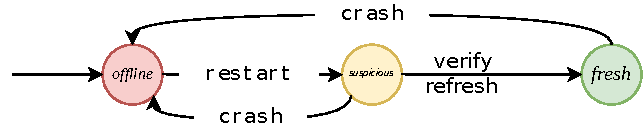
\includegraphics[width=\linewidth]{img/RR_states}
    \caption{States of a node in the \ac{RR} model. Compared
      to the crash-fault model, there is an additional ``Suspicious''
      state.}\label{fig:states}
\end{figure}

\subsection{Background: replicated systems}\label{ssec:sys_model}
\bsd{Move to related work?}

Replication protocols make a separation between clients machines
and replicas, where these two groups of nodes are connected by a
network through which any pair of nodes may communicate, defining
what is referred to as a message-passage system. These replicas
collectively implement a replicated service exporting a set of
operations, which clients may invoke. For instance, a storage
system may export a simple interface with read and write
operations, whereas a replicated database has a richer interface
supporting SQL operations. To collectively implement a replicated
service, replicas store their view of the current state of the
system that is shared among multiple clients, and client
operations are implemented by contacting a group of replicas to
either query or update that state. In general, replication
protocols leverage a ``quorum RPC'' communication
pattern~\cite{Malkhi:Reiter:BQS:98,lorenzo:framework} where a
machine (either a client or one of the replicas) sends a message
to a group of replicas and waits for a reply from a quorum. In
the fault tolerance literature, a quorum is a set of subsets of
the group of replicas, where these subsets have certain
intersection properties that are important for the protocol
correctness~\cite{gifford:quorums}. These intersection properties
depend on the fault model, e.g., with crash faults it normally
suffices that any two quorums have a non-empty
intersection~---~majorities are an example of a quorum system
with this property. Byzantine quorums, in turn, require a larger
intersection to account for incorrect replies from malicious
replicas~\cite{Malkhi:Reiter:BQS:98}.

\subsection{Replication in the \ac{RR} model}

A key insight of replication in the \ac{RR} model is to grow quorums
\emph{dynamically} when replicas are suspicious of their state.
We quantify this suspicion by counting, in each instance of the
quorum RPC pattern, how many replicas indicated the suspicious
flag, and we refer to this count as a per-RPC variable $s$.
In addition to this (dynamic) value, we also define a (static)
maximum bound on the number of nodes that may actually
suffer a rollback attack within the replica group, $M_R$.

Note that $s$ and $M_R$ are different and unrelated in several
respects. First, $s$ is measured by a node that gathers a set of
replies, and therefore its value is specific to each invocation
of an operation on a group of replicas, whereas $M_R$ is a
constant bound that is assumed to hold for that group of replicas
during the entire execution of the system. As a consequence, $s$
cannot be set at system configuration time, whereas $M_R$ needs
to be set by an administrator according to an expectation of the
deployment conditions. Second, $s$ can vary from zero (common
case, no recent replica restart) up to $N$ (simultaneous system
shutdown followed by a restart). In contrast, $M_R$ will be
parameterized according to the likelihood of a correlated
rollback attack, which in turn depends on the deployment and its
independence expectations. For example, one could deploy replicas
across different administrative domains, in which case (and
assuming that there is no collusion between administrators of
different domains), $M_R$ should be at least the maximum number
of replicas within a single domain. This encompasses the worst
non-colluding attack where a malicious administrator rolls back
all the replicas in the domain simultaneously.

Note that the parameter $M_R$ also subsumes permanent crash
faults (e.g., due to permanent hardware failure), since permanent
crashes can be seen as a particular instance of a rollback, where
we replace a failed node with a new one that starts from the
initial state of the system (or fetches a recent but possibly not
the most recent one).
%
Furthermore, we define a liveness bound $F$, i.e. the system is live
provided that no more than $F$ replicas are temporarily unreachable at
any given moment, due to network partitions, power outages, or reboot.

\subsection{Deriving {\ac{RR} Quorums}}\label{sec:parameters}

As we explained, the correctness of replication protocols hinges
on the property of quorum intersection: any pair of operations
executed in the system must execute in replica subsets (or
quorums) that intersect sufficiently for the system to return a
result that obeys the protocol specification. We now revisit this
intersection property for the design of protocols for the \ac{RR}
model. To this end, we need to first specify the set of
properties that this intersection should achieve.


\begin{property}[Freshness]
    The safety property of replicated systems normally includes
    the need for the most recently written value to be seen by
    subsequent operations. In quorum-based protocols, this
    property is enforced by ensuring that any pair of quorums
    intersects in at least one replica that does not deviate from
    its prescribed behavior. In the case of the \ac{RR} model, a
    correct replica is one that has received the most recent
    write and has not been rolled back.
\end{property}


\begin{property}[Durability]
    Durability is guaranteed if any operation that updates the
    state of the system survives any combination of faults that
    is allowed by the \ac{RR} model. In our case, this means that
    even if $M_R$ replicas are rolled back, there will be at
    least one replica with the up-to-date value.
\end{property}

\begin{property}[Operational Liveness]
    Generally, a system is live if all operations it supports eventually
    conclude.  We consider a more granular property of operational
    liveness, which separates the liveness with respect to two classes
    of operations that are normally defined in replicated systems:
    read-only (or simply read) operations, which query but do not modify
    the replicated state, and update (or write) operations that may
    operate on that state to create a new system state or simply overwrite
    it.
\end{property}

Using these properties, we place constraints on the composition
of the quorum systems. We differentiate read quorums, of size
$R_Q$, which are sufficient to conduct read operations, from
write quorums, of size $W_Q$, for write operations.

\paragraph{Freshness.}

We start by observing that, for a given read operation and within
the entire replica set, the number of nodes that could possibly
have their state rolled back is $\min(s, M_R)$. This means that a
read operation has access to a pool of replicas where $W_Q -
\min(s, M_R)$ are up-to-date and $N - W_Q + \min(s, M_R)$ may be
stale. Given that the most recent write operation contacted $W_Q$
nodes, thus bringing them up-to-date, we derive the following
minimum size for a read quorum:
\begin{equation} \label{eq:inters}
  R_Q > N - W_Q + \min(s, M_R)
\end{equation}

In our derivation, we turn the inequalities into equalities by
adding a positive (or in some cases non-negative) $\Delta$
parameter, which captures by how much each variable is larger
than strictly necessary, in this case:
\begin{align} \label{eq:inters2}
  R_Q = N - W_Q + \min(s, M_R) + \Delta_R && \Delta_R > 0
\end{align}

\paragraph{Durability.}

Additionally, we note that, since $M_R$ replicas can be rolled
back, surviving such a rollback implies that a write quorum must
include more than $M_R$ replicas, i.e.,
\begin{align}
    W_Q &> M_R \nonumber \\
    W_Q &= M_R + \Delta_W && \Delta_W > 0 \label{eq:fresh}
\end{align}

\paragraph{Write Liveness.}
We must also guarantee liveness for write operations. This
requires that a write quorum is available despite $F$ unreachable
nodes. This is guaranteed provided that:
\begin{align}
    N - F &\geq W_Q \nonumber \\
    N &= W_Q + F + \Delta_N && \Delta_N \geq 0  \label{eq:Wavail}
\end{align}


\paragraph{Final Derivation.}
The formulae above allow us to arrive at a precise formulation
for the system and quorum sizes. In particular, by
combining~\ref{eq:fresh} and~\ref{eq:Wavail}, we obtain:

\begin{align} \label{eq:ReplSize}
  N = M_R + F + \Delta_W + \Delta_N && \Delta_W > 0, \Delta_N \geq 0
\end{align}

Then, by replacing $W_Q$ (\ref{eq:fresh}) and $N$
(\ref{eq:ReplSize}) in Equation~\ref{eq:inters}, we obtain the
following equation for read quorums.
\begin{align} \label{eq:rq_size}
  R_Q = F + \min(s, M_R) + \Delta_N + \Delta_R && \Delta_R > 0, \Delta_N \geq 0
\end{align}

\paragraph{Read Liveness.}
We conduct the analysis of the liveness conditions for read
quorums separately, since these are dynamic conditions, namely
due to their dependency on the current number of possibly stale
nodes, $s$.  As such, we introduce another dynamic value: $f'$,
the number of replicas that are unreachable at any given point.
This allows us to express the dynamic liveness condition for
reads as follows:
\begin{equation} \label{eq:DynRavail}
    N - f' \geq R_Q  \Leftrightarrow f' + \min(s, M_R) \leq M_R + \Delta_W - \Delta_R
\end{equation}

This equation allows us to reason about the liveness for reads,
depending on specific runtime conditions and on how the static
parameters are chosen. For instance, we could require reads to be
live in the worst possible case of $f' = F$ and $s = M_R$, yielding
$\Delta_W \geq \Delta_R + F$.

However, this is a conservative assumption. An example of a more
realistic one would be to assume that we forfeit read liveness in
the event of a worst case level of unreachability ($f' = F$) and
there is at least one rollback ($M_R \geq 1$). This yields
$\Delta_W \geq \Delta_R + F - r$. We also choose to set
$\Delta_N=0,\Delta_R=1$ to minimize replication costs, allowing
us to derive the value for $\Delta_W$ from
Equation~\ref{eq:DynRavail}:
\begin{align} \label{eq:deployment1}
  \Delta_W &\geq  \Delta_R + F - M_R\\
  \Delta_W &\geq  1 + F - M_R
\end{align}

When also taking into account that $\Delta_W > 0$, and turning
the inequality into an equality to minimize replication costs,
this allows us to derive:
\begin{align} \label{eq:deployment2}
  \Delta_W &=  \max(1,1 + F - M_R)\\
  \Delta_W &=  1 + \max(F - M_R,0)
\end{align}

This results in these possible deployment parameters:
\begin{align} \label{eq:deploymentfinal}
    N &= \max(M_R, F) + F + 1  \\
    W_Q &= \max(M_R, F) + 1 \\
    R_Q &= F + \min(s, M_R) + 1 \label{eq:proof3}
\end{align}

\paragraph{Atomic update operations.}
As we mentioned, more complex systems such as replicated
databases, instead of following a simple read/write interface,
support rich operations that read the most recent value of the
system \emph{and} update it with a new value derived from the
value that was read. To achieve this, their protocols may need to
gather both a read and write quorum (i.e., $\max(R_Q, W_Q)$
replies). We dub these quorums \emph{super quorums} and use $S_Q$
to represent their size.

\paragraph{Quorum properties.} This derivation of the various quorum
sizes leads to the following set of properties that \ac{RR} quorum
systems obey (also illustrated in Figure~\ref{fig:quorums}):

\begin{enumerate}
    \item[\textbf{I1.}] Any read quorum intersects with any write
        quorum in at least one replica whose state was not rolled
        back;
    \item[\textbf{I2.}] It is possible some pairs of read quorums
        do not intersect.
\end{enumerate}

Using these properties, we can derive the following
property of super quorums:

\begin{enumerate}
    \item[\textbf{I3.}] The intersection between a super quorum
        and a quorum of any other type is non-empty and includes
        a replica whose state has not been rolled back.
\end{enumerate}

These properties, along with the fact that read quorums can be
smaller than write quorums in the normal case when there
are no restarts, play a role in the design and performance of
protocols in the \ac{RR} model, as we will see next.

\begin{figure}[t]
    \centering
        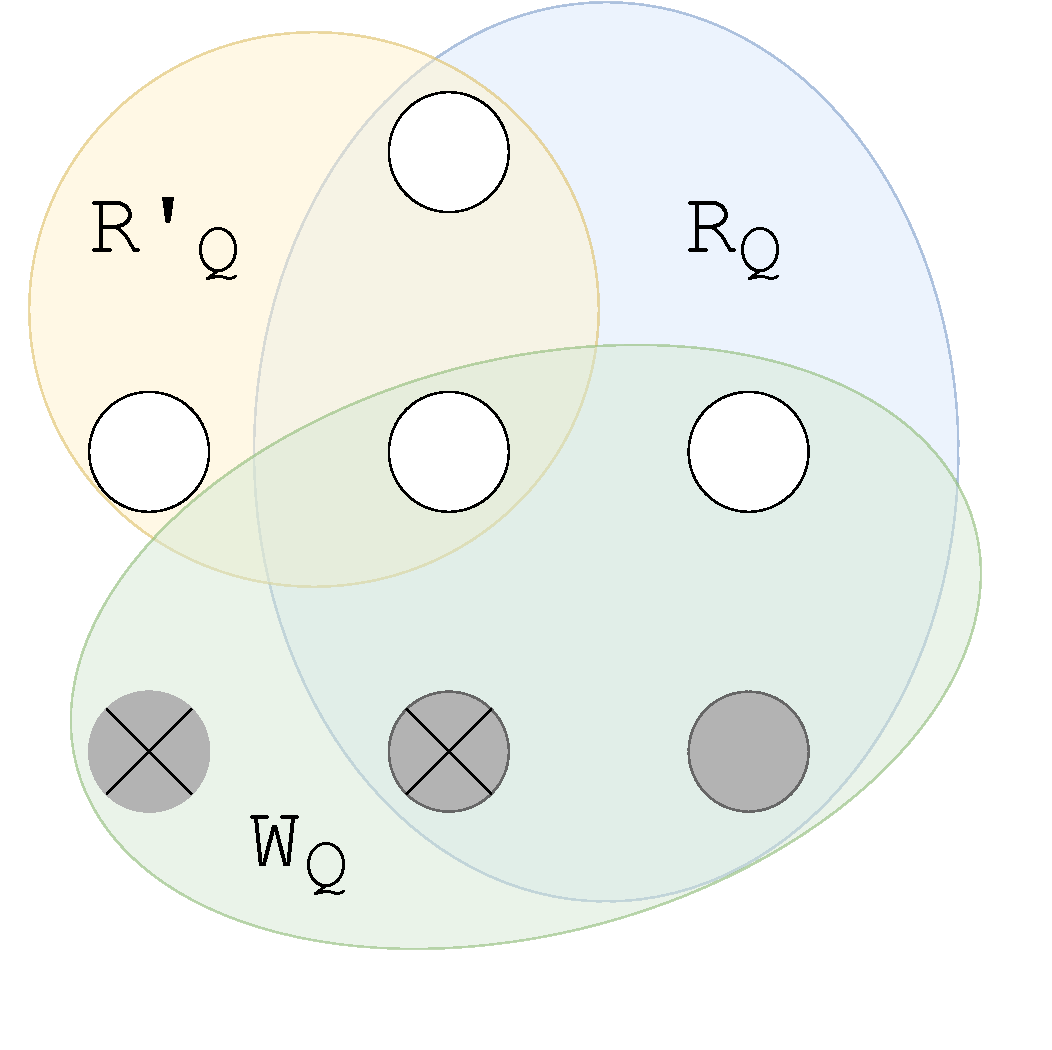
\includegraphics[width=.32\linewidth]{img/RR_quorums_I1}
        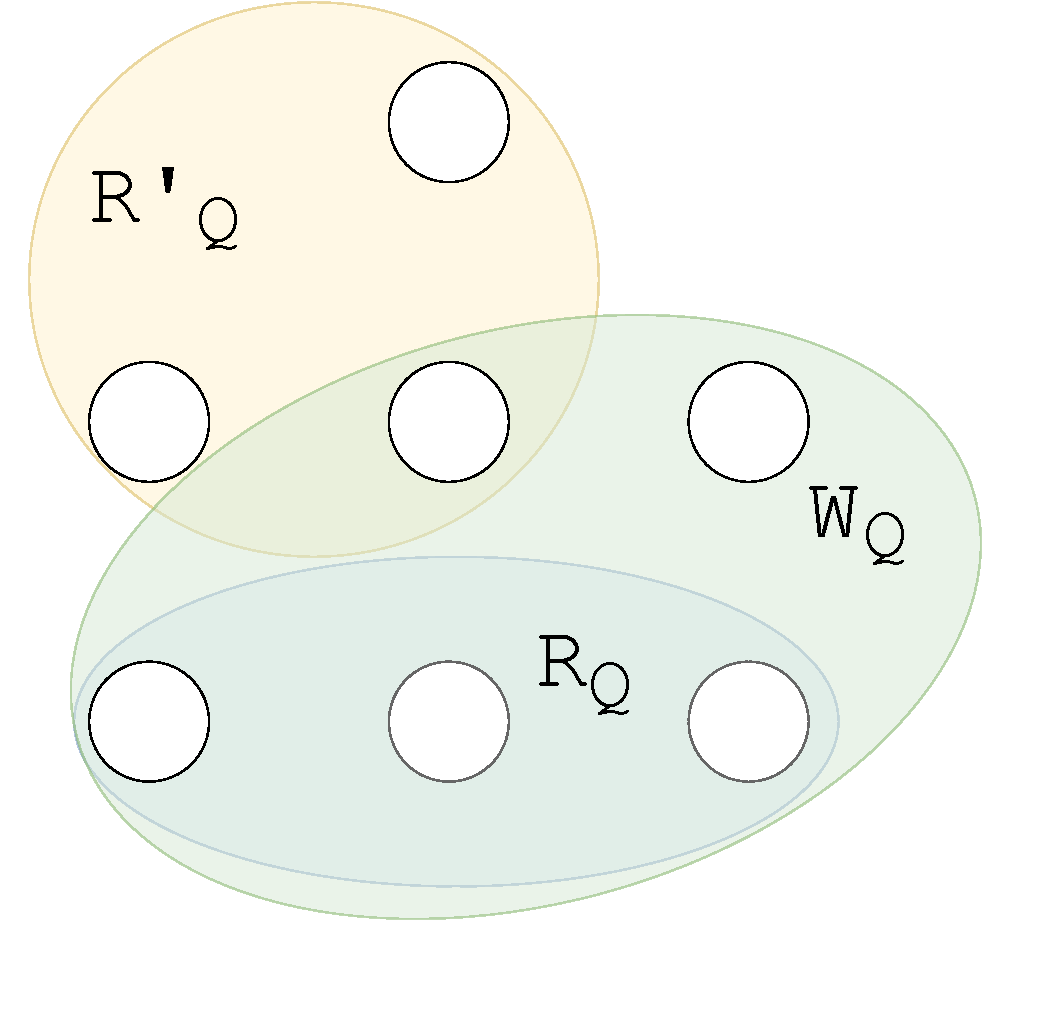
\includegraphics[width=.32\linewidth]{img/RR_quorums_I2}\\
        (a) \hspace{2.3cm} (b) \hspace{.2cm}
    \caption{Example of a \ac{RR} quorum system ($M_R=4$,
    $F=2$). In (a), there were $3$ restarts (shaded) and $2$ rollbacks
    (crossed). Thus, the read quorum receives suspicious replies and
    grows larger, ensuring that both read quorums still intersect $W_Q$ in
    at least one up-to-date replica (as required by \textbf{I1}).
    In (b), there are no restarts (and, by extension, no
    suspicion of rolled back state), and thus read quorums can be
    disjoint, as noted by \textbf{I2}.}\label{fig:quorums}
\end{figure}

\paragraph{Reflections on the parametrization of the system.}
\ac{RR} quorums are more complex than regular
quorum systems. They include two parameters ($M_R$ and $F$) instead of
one, with an additional runtime value ($s$). Moreover, the quorum
system is inherently asymmetric, leading to three different types of
quorums (read, write, and superquorums), as opposed to a single one.
This puts a burden on the system designer to use the right type of quorums for
different protocol steps, and also, at deployment time, to consider how to
choose $M_R$ (to represent the anticipated maximum number of simultaneous rollback
attacks on the system), and $F$
(to encode the availability of the system, by estimating how many replicas
can crash without jeopardizing liveness).
%
However, we believe that this complexity is warranted, not only
because it is naturally derived from the nature of the faults (in
particular, the fact that it is possible to determine precisely when a
replica is or is not susceptible to a rollback of its persistent
state), but also because it allows us to extract the maximum
performance from the system and avoid wasting resources used in
replication.

\bsd{TODO: classify the two types of quorum systems}.

\paragraph{Comparison with existing asymmetric quorum schemes.}

Previous proposals for asymmetric quorum schemes differ
significantly from \ac{RR} quorum systems.  The idea of
asymmetric quorums dates back to one of the initial proposals for
quorum systems by Gifford~\cite{weighted_voting}, where a
replicated object has a certain number of votes and in order to
read the value, $M_R$ votes must be gathered, whilst $w$ votes
are required to write the value. The equivalent to the
intersection property \textbf{I1} is guaranteed by ensuring that
$r + w$ exceeds the total number of votes of the object. This use
of asymmetric quorums has also been motivated by different goals.
In particular, asymmetric quorums have been proposed in the
context of asymmetric trust assumptions~\cite{asymmetric_trust},
where each node makes its own assumptions about which nodes might
be Byzantine. Another type of use of asymmetric quorums is to
obtain better performance, by making the commonly used quorums
smaller than the ones that are used less
often~\cite{fp,wheat,rqs} or reducing the asymptotic complexity
of quorums at the expense of more replicas~\cite{grid_quorums}.

Compared to these approaches, \ac{RR} quorums are derived from
the dynamic nature of the number of possible rollbacks that are
present in the system at any given moment. This natural
construction leads to interesting properties of the system,
namely allowing for performance to improve in the normal case
when there are no recent replica restarts, due to the use of
relatively small read quorums.

\section{Replication protocols}\label{sec:protocol}

Designing and implementing new replication protocols, as well as
proving their correctness, is a non-trivial effort. Consequently,
rather than building protocols for the \ac{RR} model from
scratch, we propose a set of principles for adapting existing
protocols to the fault model. In this section, we identify
principles for this adaptation and apply them to existing
protocols, showing that the adaptation is straightforward.

\subsection{Principles and challenges for protocol adaptation}

When adapting existing protocols to the \ac{RR} model, it is
convenient to start from a crash fault tolerant protocol.
Due to the \new{correctness of execution of nodes in the \ac{RR}
model}, nodes observe mostly crash fault behavior; the only
additional fault behavior is that their externally stored state
may be stale after a restart.

Most replication protocols are quorum-based, where a client (or a
replica acting on behalf of a client) needs to obtain responses
from the quorum or replicas to perform an operation.  Therefore,
an important aspect of adapting a crash fault tolerant protocol
consists of following the quorum sizes defined in
Section~\ref{ssec:parameters}. Similarly, reconfiguration is a
key aspect of practical replication protocols. Quorum sizes for
these reconfiguration protocols also need to be adapted
accordingly.

Each node must be augmented to maintain a suspicion flag. When a node
restarts, it set the suspicion flag to true. At this point, the node
runs a recovery subprotocol (eagerly or lazily), which is not required
in the crash model.

While the recovery subprotocol is dependent on the specifics of
the protocol being modified, the general method is as follows. On
restart, a replica queries a read quorum of replicas for a digest
of their state, retaining the replies that contain the most
recent state, e.g., determined through timestamps as exemplified
next.  From this read quorum of digests, it can determine the
digest of the current system state, and check whether its state
is up-to-date, thus clearing the suspicion flag. If not, then the
specific parts of the state that are stale need to be fetched
from other replicas to bring the recovering replica up-to-date.
To efficiently find which elements of the state are out of date,
replicas may maintain a Merkle tree, which allows for determining
which parts of the state need to be fetched without transmitting
a large amount of information. Note that this subprotocol can run
lazily and in the background, while the replica continues
satisfying requests. Doing so might allow for clearing the
suspicion flag in case of an update where the new state does not
depend on the previous version.

Finally, if the adapted replication protocol is to be configured such
that $F<M_R$, read quorums may not intersect (see quorum property
\textbf{I2} in Section~\ref{ssec:parameters}).  Here, two disjoint
read quorums may ion general reflect different system states~---~a
phenomenon usually described as {\em split brain}.  This can happen
when an operation that changes the system state is still in progress
(or even halted, due to the crash of the initiator). When adapting
protocols, designers must take this into account and implement
mechanisms to ensure that a single value is reported by all read
quorums, if required.

Next, we will present two example protocols that follow these
principles and illustrate some of the above challenges.

\subsection{Read-write register}\label{ssec:abd}

In this section, we present an adapted version of the ABD~\cite{abd}
protocol for a distributed read/write register with linearizable
semantics\footnote{A concurrent object is
linearizable iff there exists a serialization of all operations
which is equivalent to a sequential execution and the
serialization matches the real-time order of invocation/reply.}~\cite{linearizability} under the \ac{RR} model. ABD provides a simple
read/write interface, which is useful for storage systems or services
that offer a read/write interface. Read/write register protocols have
the advantage of guaranteeing termination even in asynchronous systems
with faults, and having good performance due to a simple message
pattern that is linear in the number of replicas~\cite{gryff:nsdi20}.
%
Figure~\ref{fig:abd-read} shows the pseudocode for the read operation
while the write logic is shown in Figure~\ref{fig:abd-write}. Since
the code follows closely the original ABD protocol, our
explanation highlights where we adapted the protocol to the
new fault model.

\paragraph{Timestamp Structure.}
Each data item stored is associated with a
timestamp, which defines the linearization order of the version
that is stored. Timestamps have two numeric components $\langle
seqno, client\_id \rangle$, where $client\_id$ is the
unique, ordered id of the client issuing the write.  This
breaks ties when two clients write different values to the same
sequence number.
%Additionally, there is a $stable$
%boolean flag, associated with the timestamp, indicating whether
%the vallue is stable or not.

\paragraph{Write.}  This operation is similar to the ABD
protocol, but uses the \ac{RR} quorum system. In the first round
a read quorum is gathered to discover the most recent sequence number
(the one associated with the highest timestamp).  In the second round,
that sequence number is incremented by the client, appended with the
client id, and the resulting timestamp is sent with the value to be
written. Upon receiving this second round message, replicas overwrite
values if the received timestamp is greater than the one associated
with the data they store.


\paragraph{Read.} Following the ABD protocol, reads occur in one
round in the common case, with a second round being required if a
value needs to be written back. In particular, in the original ABD
protocol, the first round queries replicas for their data and
timestamp, waits for replies from a majority (which equates to both a
read and write quorum) and the return value corresponds to the reply
with the highest timestamp. However, when there is no majority that
holds that timestamp value, the second phase is required, writing this
timestamp and data to a majority. (This is needed to conclude a write
operation that executes concurrently or was left unfinished.)

Translating the notion of a majority to read and write quorums in the
\ac{RR} model presents a subtle challenge. Even though
intuitively the initial read round only requires a read quorum (and in
fact this is sufficient to determine the read reply), the optimization
of skipping the second round is only applicable if there is unanimity
for that timestamp in a write quorum. This is because read quorums do
not necessarily intersect (property \textbf{I2}), which implies that
contacting only a read quorum would allow for a ``split brain''
situation, where clients read different values depending on which
quorum they contact, thus breaking linearizability. The problem with
waiting for a larger quorum, however, is that in scenarios
where inter-node latency has a wide variance such as geo-replication,
this introduces an additional latency that erodes the performance
advantage of the smaller quorums.% in the \ac{RR} model.
%We address this through a stabilization phase described next, which is useful beyond the use of this fault model, namely to asymmetric non-intersecting quorums in crash fault tolerant protocols.

%% Although having an ultimately protocol-dependant solutions, the
%% approach is common. The split-brain situation described above is
%% always a result of an in-progress write, meaning we need to
%% identify when this situation is actually occuring and employ
%% mechanisms to make sure that only one of the disjoint
%% read-quorums can return a value (and the other read operations
%% would need to fall back on larger quorums).

\begin{figure}[t]
  \begin{small}
    \textbf{Read} at client $c$

    \begin{enumerate}[itemsep=0pt,parsep=0pt]

    \item \textbf{send} $\textsc{read-replica}$ to all replicas

    \item \textbf{wait until} received  \textbf{either} $R_Q$ replies, such that, for the highest timestamp $ht$, $ht.stable==\textsc{true}$
       \textbf{or until} received $W_Q$ replies where the highest timestamp has $ht.stable==\textsc{false}$

    \item \textbf{if} $ht.stable==\texttt{true}$ \textbf{then}\\
        \tabto{.5cm}   \textbf{return} $\textsc{success}(ht,val(ht))$

    \item \textbf{if} $\exists W_Q$ of replies with $ht$ \textbf{then}\\
        \tabto{.5cm} \textbf{send} $\textsc{stabilize}(ht)$ to all replicas;\\
        \tabto{.5cm} \textbf{return} $\textsc{success}(ht,val(ht))$
    \item \textbf{send} $\textsc{write-replica}(ht,val(ht))$ to all replicas
    \item \textbf{wait until} received $W_Q$ of \textsc{success} replies

    \item \textbf{send} $\textsc{stabilize}(ht)$ to all replicas
    \item \textbf{return} $\textsc{success}(ht,val(ht))$

    \end{enumerate}

  \end{small}
  \caption{Pseudo-code for the register read operation.}\label{fig:abd-read}
\end{figure}

\begin{figure}[t]
  \begin{small}
    \textbf{Write (value $v$)} at client $c$

    \begin{enumerate}[itemsep=0pt,parsep=0pt]

    \item \textbf{send} $\textsc{read-replica}$ to all replicas

    \item \textbf{wait until} received $R_Q$ replies

    \item \textbf{let} $ht$ be the largest timestamp in quorum

    \item \textbf{let} $new\_ts$ be $\langle ht.seqno + 1, c, \texttt{false}\rangle$

    \item \textbf{send} $\textsc{write-replica}(new\_ts,v)$ to all replicas

    \item \textbf{wait until} received $W_Q$ \textsc{success} replies

    \item \textbf{send} $\textsc{stabilize}(ht)$ to all replicas
    \item \textbf{return} $\textsc{success}$
    \end{enumerate}

  \end{small}
  \caption{Pseudo-code for the register write operation.}\label{fig:abd-write}
\end{figure}

\paragraph{Stabilization.}
To address this issue, we introduce an extra asynchronous phase,
called the \emph{stabilization} phase. This phase takes
place in the background after a value has been successfully
written to a write quorum (either in a write operation or in the
writeback phase of a read operation), without
blocking the operation from returning to the client. A
\textsc{stabilize} message is sent to the replicas so that they
will set a \emph{stable} flag associated with the recently
written timestamp and value. Since this is an optimization, there
is no need for replicas to reply to this message.  Marking a
value as stable means that the write operation for this value has
concluded (i.e., reached a write quorum), which implies that all
read quorums include at least one replica that will report either
this or a newer value, given that a write quorum intersects all
read quorums (\textbf{I1}). Therefore, in the first phase of the
read operation, if the most recent value in a read quorum is
marked stable, even if it is read from a single replica, it can
be immediately returned, since the stable flag indicates that it
has been written to a write quorum and will therefore be seen by
any subsequent read quorum, thus obeying linearizable semantics.

The stabilization phase can
occur at any point after the write concludes. Considering an eager
approach, the stabilization would occur right after the value has been
written. We follow a lazier option, triggering the stabilization only
after the first read (thus avoiding stabilizing a value which is never
read).

\paragraph{Proof sketch.}
We prove the correctness of the resulting protocol in the
appendix, and sketch here a correctness argument. The proof of
linearizability of a read/write object follows a helper
theorem~\cite{nancy-book}, requiring, for any execution, the
existence of a total order that is both consistent with the
results the operations return and consistent with the real time
order of request invocations and replies. In our proof, this
total order is established by the timestamp order (in case of
operations with the same timestamp, reads follow both writes and
other reads that precede them in real time order).  Then we prove
that this meets both consistency requirements above: for the
output of reads, this is by construction due to reads being
ordered after the corresponding writes; then,
the consistency with the real time request order follows from the
fact that the quorum intersection property \textbf{I1} from
Section~\ref{sec:model} implies that reads see the effects of
previously completed reads or writes either directly, because the
preceding operation contacted a write quorum, or indirectly, via
the stable flag.


\subsection{State-machine replication}\label{ssec:paxos}

State machine replication (SMR) allows for replicating any
deterministic service by enforcing that operations are executed in the
same order on all replicas. Paxos~\cite{paxos} is the best known
instance of this paradigm, but there are several different
descriptions, with little consensus on what the exact Paxos protocol
entails.  Since our goal is to showcase the changes required by the
\ac{RR} model, we chose as a starting point the versions that
describe the persistent state that is logged at each protocol
step~\cite{paxos_builders,paxos_engineering}. In contrast, most other
Paxos descriptions only store the replica state in memory, and therefore
do not allow, for instance, the simultaneous restart of all the
replicas --- only up to $F$ of them can restart at a time. We next
present the adaptation of this protocol to \ac{RR}, focusing on
the normal case operation for conciseness.

\begin{figure}[t]
  \begin{small}
    \textbf{Execute (operation $op$)}

    \begin{enumerate}[itemsep=0pt,parsep=0pt]

        \item \textbf{client\_send} $\textsc{execute}(op)$ to \emph{leader}

        \item \textbf{leader} assigns slot number $s$ to $op$

        \item \textbf{leader\_broadcast} $\textsc{prepare}(s, op)$, after logging to disk

        \item \textbf{replica\_broadcast} $\textsc{accept}(s, op)$, after logging to disk

        \item \textbf{wait until} $\#accepts(s) \geq S_Q$, marks $op$ as accepted
    \end{enumerate}

  \end{small}
  \caption{Pseudo-code for the normal case SMR operation.}\label{fig:smr-update}
\end{figure}

\begin{figure}[t]
    \centering
    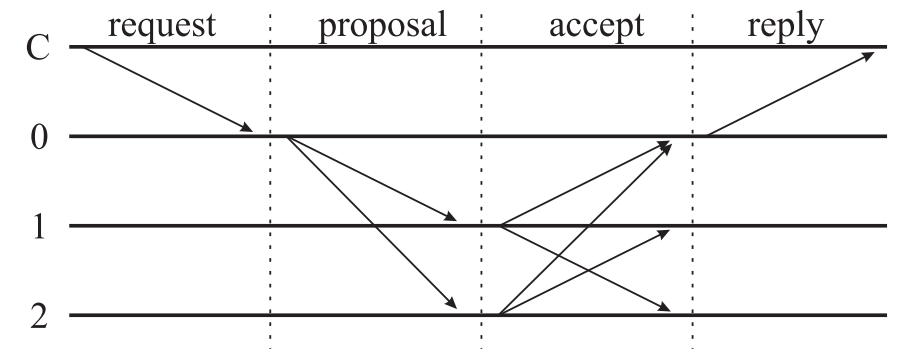
\includegraphics[width=.65\linewidth]{img/paxos}
    \caption{Diagram of a normal case SMR operation}\label{fig:paxos}
\end{figure}
\paragraph{Normal case operation.}
We follow the multi-Paxos protocol~\cite{paxos_simple,paxos_engineering},
where there is
a component of the protocol that elects a stable leader replica, guaranteeing
that only that replica can propose the sequencing of new operations while
it remains the leader. That sequencing corresponds to the normal case
operation, which is described in the pseudocode in
Figure~\ref{fig:smr-update}, and is depicted in
Figure~\ref{fig:paxos} (following the protocol
description from~\cite{paxos_builders}). In summary, the leader replica
proposes a sequence number for incoming client requests, and this sequencing
must be accepted by a quorum of replicas (a majority in Paxos), who validate
that this sequence number had not been assigned yet. Once
such a majority is gathered, replicas execute the client operation in that
order and the leader replicas replies with the output of the operation
to the client.

\if 0
\begin{enumerate}
    \item A client sends the operation $op$ to be executed to the leader;
    \item The leader assigns the operation a slot number $s$ on the
      sequence of state machine commands (based on the next free slot in
      its local sequence);
    \item The leader sends $prepare(s, op)$ to all replicas,
        logging the sending of this message in persistent storage
        before initiating its transmission;
    \item If a replica has slot $s$ open in its sequence of commands, it sends an
        $accept(s, op)$ to all replicas, also logging the accept
        message persistently before sending it.
    \item A replica marks a slot as accepted when it receives
      the $S_Q$ matching accepts for that slot.
\end{enumerate}
\fi

Our protocol follows directly from this protocol
description~\cite{paxos_builders}, modifying only the quorum size
when gathering the quorum of accept messages. When moving from
majoriy quorums to the separate quorum
types, we need to observe that a Paxos round is both reading and writing
the current state of the Paxos protocol. This is because it must
read that the slot that is being proposed is not yet taken, and
at the same time record the fact that the slot becomes taken and
cannot be used in subsequent proposals. Thus, majorities are
replaced with superquorums in the \ac{RR}-tolerant version of
Paxos.


\paragraph{Leveraging the \ac{RR} model.}
So far, the protocol adaptation does not leverage the
small read quorums enabled by the \ac{RR} model. Even
read-only operations are serialized in the state machine, and as
such need to update the system state, namely to fill the position
in the sequence of operations.

To leverage small read quorums, we adapt the read-only
optimization described in some protocols such as PBFT~\cite{pbft} or
the Paxos description by van Renesse and Altinbuken~\cite{pmmc}.  In
this optimization, the client contacts a read quorum with an
\textsc{optimized-read} message, asking for the
result of executing the read-only command against current state of the
replicas. If the replies are unanimous, the client can return the
value.

Applying this optimization requires careful reasoning to avoid
violating the linearizable semantics of the protocol. To
understand why, consider the possibility of two successive read
operations, $r_1, r_2$, where $r_1$ ends before $r_2$ begins, and
that use quorums $Q_{R1}$ and $Q_{R2}$ (respectively) and execute
concurrently with a write $w$ that gathers a quorum of accepts
$Q_W$. In this case, and given property \textbf{I2} (read quorums
may not intersect), $r_1$ may see $w$ as being complete in a read
quorum, but $r_2$ only contains replicas that have not yet
gathered a write quorum of accepts for $w$, since those replicas
might have sent but not yet received the necessary number of
accepts. This would violate linearizability since $r_1$ precedes
$r_2$ in real time but, given their outputs, they cannot be
linearized in that order.

This is yet another occurrence of a split brain scenario, but
the solution in this situation is different: instead of
confirming a written value via stabilization, we abort the
optimized read when it is possible that another value has been
written to the state machine, falling back to reading using a
state machine operation. A replica can detect this situation if
it has sent an $\textsc{accept}$ message for a slot
higher than the last executed operation (as it indicates the
possibility of another read quorum with a different value). If no
replicas in a read quorum have done this, then no other operation
has concluded (\textbf{I1}).

\paragraph{Proof sketch.}
Just as in the \ac{ABD} protocol, we sketch the proof based on
the existence of a total order for the operations that is
consistent with both the output of operations and the real time
order of request execution and replies~\cite{nancy-book}. This
total order is built in the same manner as before, i.e., it is
given by the slot number $s$, breaking ties by having read-only
operations succeeding both the most recent read/write operation
reflected in the reply and read-only operations with the
same slot number that precede them in real time. By the
construction of the protocol, this order is consistent with the
results that are output to the client, since the replies reflect
the execution of the preceding sequence of state machine commands.
The proof for that the order is consistent with
the real time order of requests is straightforward for the
non-optimized protocol but more subtle for the case where one or
both of the requests follow the read-only optimization.
In this case, a later read-only operation cannot revert to a
previous state because of the protocol feature that replicas with
pending accepts deny an optimized read.  This ensures that
it is impossible to have a more recent state
that could have been reflected by a preceding read/write or
optimized read, because intersection property \textbf{I1} implies
that at least one node from the read quorum in the later read
would have sent the accept for the operation that created the
more recent state, since its execution requires a write quorum of
accepts.


\subsection{Security Properties}\label{ssec:sec_prop}
\bsd{Consider moving to chapter 4}
If the threat model for \acp{TEE} explained in
Section~\ref{sec:fault_model} holds, the protocols described in this
section achieve freshness, integrity and confidentiality.
Confidentiality of the overall system is inherited trivially from the
\ac{TEE} fault model. Integrity and freshness of data follow from the
correctness of the protocols, guaranteed by their linearizability
proofs (present in full in the Appendix). These proofs rely on
the intersection properties of the quorum system, in particular
that they mask the rolled back replicas. Moreover, they assume the
\ac{RR} model applies to the replicas, which is
guaranteed by encapsulating replicas inside the \acp{TEE}. Crucially,
the usage of \acp{TEE} (which have integrity of the computation)
guarantees that the protocol is followed by all replicas (even if
they have stale data).

\section{Evaluation of \ac{TEE} replication protocols}

We evaluate our various implementations based on the \ac{RR}
model using micro-benchmarks for protocol implementations and
benchmark workloads for the full system built using those
protocols. Our experiments attempt to answer the following
questions:

\begin{enumerate}
    \item How significant is the effort to change a \ac{CFT}
        implementation to support the \ac{RR} model?
        (\S\ref{ssec:implementation_effort})
    \item How do the protocols based on the \ac{RR} model
      compare with their counterparts based on the Crash and Byzantine
      fault models? And how does that performance behave under increased load?  (\S\ref{ssec:eval_quorum})
\end{enumerate}

\subsection{Implementation}\label{ssec:impl}

We implemented both the read/write register and SMR protocols in
the three fault models (crash, \ac{RR}, and Byzantine) in Intel
SGX (version 1), using C++. All prototypes were implemented using
the same codebase, limiting the changes between prototypes to
what was required by the protocols (e.g.\ extra protocol steps,
different quorums). The PBFT~\cite{pbft} implementation uses the
standard optimization of using MACs instead of digital
signatures.

SGX applications have two separate regions of memory: the
application (untrusted) and the enclave (trusted). In all cases,
the application code comprises 1KLoC (mostly for bootstrap and
interfacing with the local \ac{OS}). All replicas are implemented
using a single-threaded event loop, and take between 4.5KLoC for
the distributed register and 4KLoC for \ac{SMR}. Additionally, the client libraries, which
interact with the replicas take up 5KLoC (distributed
register) and 4KLoC (\ac{SMR}).

It is important to observe that, since in the \ac{TEE} use case,
replicas cannot generally trust clients to execute the protocol
code correctly, our prototypes implement the driver code
collocated with the replicas. This is only relevant in the
distributed register case, since there is no client-side protocol
to be executed in Paxos. A possible alternative would have been
to implement a \ac{TEE} library that drives the register
protocol, which all replicas would remotely attest. We chose
not to do this, since this approach has wider applicability
(e.g.:\ it allows clients that do not run in \ac{TEE}-enabled
platforms to interact with a \ac{TEE} replicated system).

\subsection{Evaluation}\label{sec:eval}

\bsd{TODO, revert back to linewidth}
\begin{figure*}[th!]
    \centering
    \begin{subfigure}[t]{0.24 * 10cm}
        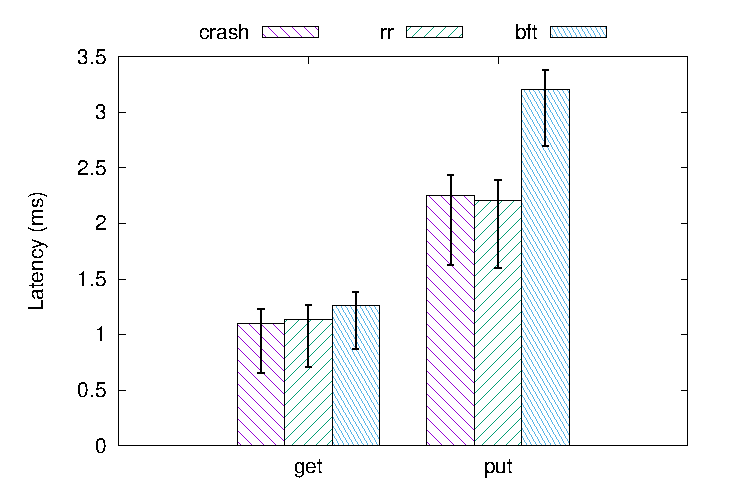
\includegraphics[width=\linewidth]{teem_results/protocol/1ms/lat/1ms_reg}
        \caption{Read-write register ($1ms$)}\label{fig:1ms_reg_lat}
    \end{subfigure}
    \begin{subfigure}[t]{0.24 * 10cm}
        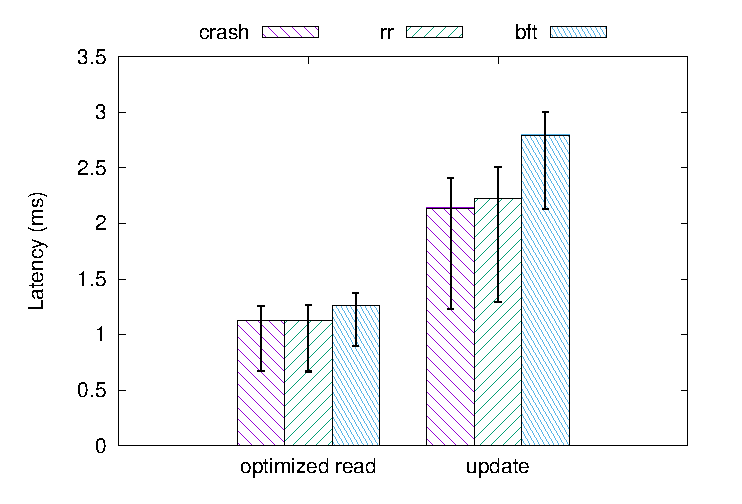
\includegraphics[width=\linewidth]{teem_results/protocol/1ms/lat/1ms_smr}
        \caption{State machine ($1ms$)}\label{fig:1ms_smr_lat}
    \end{subfigure}
    %\vskip 0.1cm
    \begin{subfigure}[t]{0.24 * 10cm}
        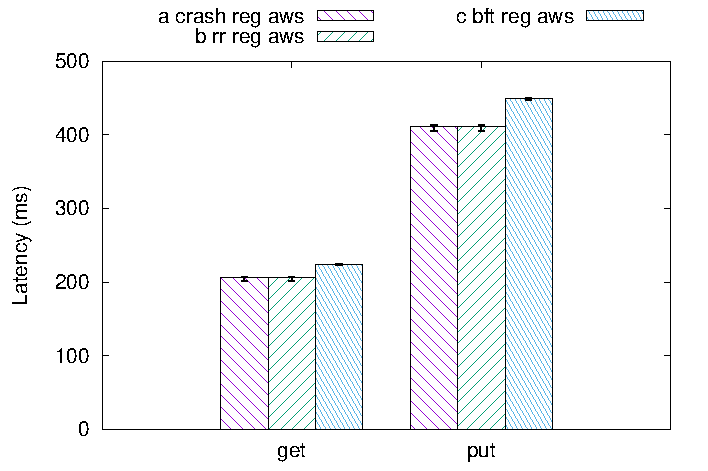
\includegraphics[width=\linewidth]{teem_results/protocol/aws/aws_reg}
        \caption{Read-write register (AWS)}\label{fig:aws_reg_lat}
    \end{subfigure}
    \begin{subfigure}[t]{0.24 * 10cm}
        \centering
        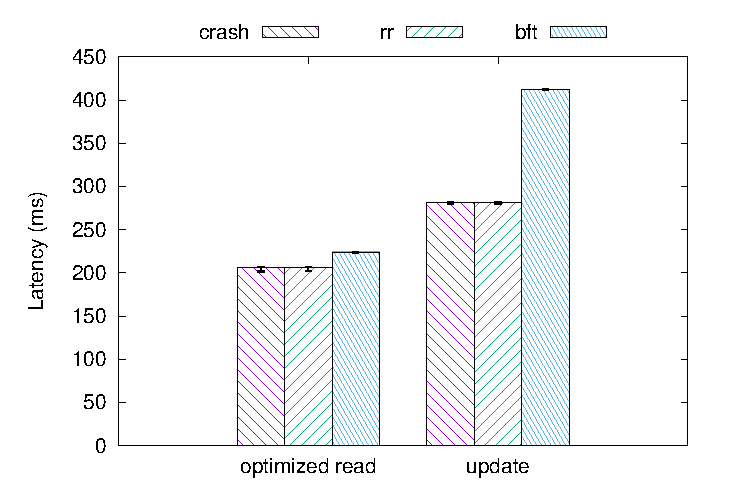
\includegraphics[width=\linewidth]{teem_results/protocol/aws/aws_smr}
        \caption{State machine (AWS)}\label{fig:aws_smr_lat}
    \end{subfigure}
    \caption{Operation latency for different protocols in
    different network topologies}
\end{figure*}\label{fig:protocol_lat}

\bsd{TODO, revert back to linewidth}
\begin{figure*}[th!]
    \centering
    \begin{subfigure}[t]{0.45 * 10cm}
        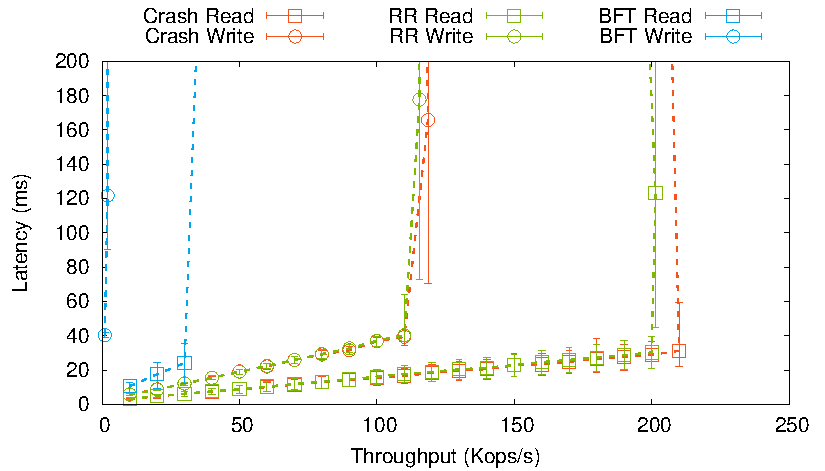
\includegraphics[width=\linewidth]{teem_results/protocol/1ms/reg-tput/result/reg}
        \caption{Read-write register}\label{fig:reg_tputlat}
    \end{subfigure}
    \begin{subfigure}[t]{0.45 * 10cm}
        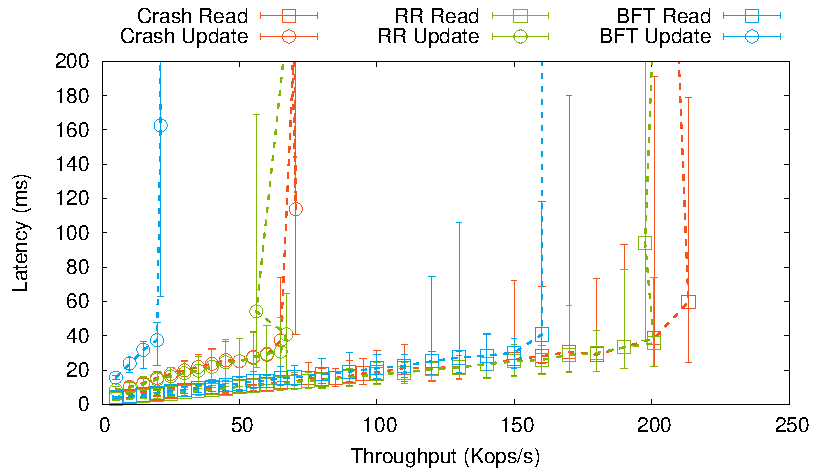
\includegraphics[width=\linewidth]{teem_results/protocol/1ms/smr-tput/result/smr}
        \caption{Replicated state machine}\label{fig:smr_tputlat}
    \end{subfigure}
    \caption{Throughput-Latency curve for different protocols}
\end{figure*}

\noindent \textbf{Experimental Setup.}
We ran our experiments using 7 machines  with
Intel$^\text{\textregistered}$ Xeon$^\text{\textregistered}$ E-2174G
processors running Debian Linux version 4.19 to run the replicas,
plus 2 machines equipped with Intel$^\text{\textregistered}$
Xeon$^\text{\textregistered}$ Platinum 8260M processors running Debian
Linux version 5.4: one of them to execute the clients and the other to
host Redis.
%
All machines were connected to same local network. To emulate
different deployment scenarios, we developed
\texttt{sloth}\cite{sloth}, which internally uses
\texttt{netem}\cite{netem} to implement a network topology from a
high-level JSON description. We considered two deployment
scenarios in these experiments: a local area network where all
machines are connected by links whose latency follows a normal
distribution with mean $1$ms and standard deviation of $\sigma =
0.5$ms (which we will refer to as the $1$ms topology); the
deployment scenarios of Figure~\ref{fig:deployments}; and a
geo-replication scenario, based on the measured the link
properties (latency and bandwidth) between several AWS
EC2~\cite{ec2} instances (t2.medium or t3.medium types), located
in regions spread across the globe (AWS topology). This setup
ensures flexibility and experimental reproducability.

In our result graphs, each data point represents the median
measurement over $3,000$ requests (except throughput numbers as
described belows) and the error bars show the $5^{\text{th}}$ and
$95^{\text{th}}$ percentiles.

\subsection{Code changes}\label{ssec:implementation_effort}

Changing a \ac{CFT} implementation to reflect the protocol changes
required by the \ac{RR} model requires low programming
overhead. Mainly, the adaptation needs to handle the restart
flag, the existence of different quorums and the mechanisms to
prevent split brain. For the read/write register prototype, we
modified $72$ LoC and added $211$ new ones. For the SMR
prototype, we modified $24$ LoC and added $28$.

\bsd{TODO, revert back to linewidth}
\begin{figure}[t]
    \centering
    \begin{subfigure}[t]{.49 * 10cm}
        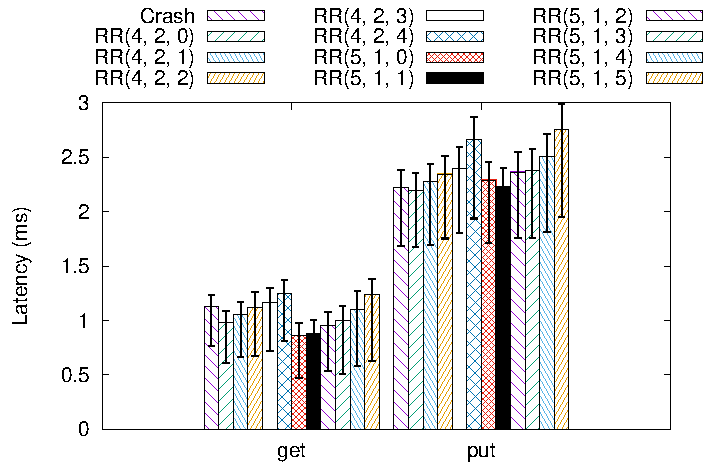
\includegraphics[width=\linewidth]{teem_results/protocol/1ms/parameter/reg_parameter}
        \caption{Read-write register}\label{fig:1ms_reg_lat_conf}
    \end{subfigure}
    \begin{subfigure}[t]{.49 * 10cm}
        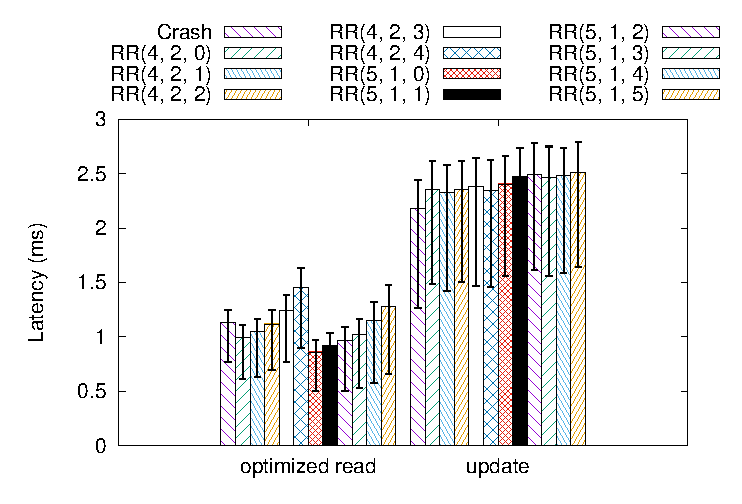
\includegraphics[width=\linewidth]{teem_results/protocol/1ms/parameter/smr_parameter}
        \caption{State machine}\label{fig:1ms_smr_lat_conf}
    \end{subfigure}
    \caption{Latency for
    different configurations and models in the $1$ms topology. \ac{CFT} uses
    $F=3$ and $RR(M_R, F, s)$ denote \ac{RR} with parameters $M_R$ and
    $F$, with $s$ restarts.}
\end{figure}\label{fig:protocol_parameter_lat}


%-------------------------------------------------------------------------------
\subsection{Protocol performance in different models}\label{ssec:eval_quorum}
%-------------------------------------------------------------------------------

Next, we focus on comparing the performance of both classes of protocols under different
fault models.
%
We compare our adaprted read-write register with the original ABD
protocol and the \ac{BFT} read-write register protocol described
in~\cite{Malkhi:Reiter:BQS:98}. For SMR, we compared our protocol with
Paxos as described by Kirsch and Amir~\cite{paxos_builders} and the
PBFT protocol~\cite{pbft}. We fixed the fault parameter, $F= 2$ across
quorum systems (with $M_R=2$ in the \ac{RR} quorum system),
yielding quorums with $3$ replicas in the crash and
\ac{RR} models and $5$ replicas in the Byzantine model. The
parametrizations are summarized in
Table~\ref{table:quorum_sizes}.

\begin{table}[b]
    \centering
    \begin{tabular}{|r || c | c | c || c | c |}
        \hline
        \textbf{Model}       & N & F & M$_R$ & R$_Q$ & W$_Q$\\ \hline
        \textbf{\ac{CFT}}         & 5 & 2 &   &   3   &   3  \\
        \textbf{\ac{RR}} & 5 & 2 & 2 &   3   &   3  \\
        \textbf{\ac{BFT}}         & 7 & 2 &   &   5   &   5  \\ \hline
    \end{tabular}
    \caption{Parameters required by different fault models.}\label{table:quorum_sizes}
\end{table}

Table~\ref{table:quorum_sizes} summarizes the protocol parameters,
which were chosen to tolerate the same number of faults across
systems, and the resulting quorum and system sizes.

The results in Figures~\ref{fig:1ms_reg_lat}-~\ref{fig:aws_smr_lat}
reflect the differences between the different fault models.  We
observe that larger quorums make the operations slower, since the
operation latency is bound by the latency of the slowest replica in
the quorum. Notably, in both cases the performance of the
\ac{RR} protocols matches that of the \ac{CFT} ones, which is to be
expected as they have equally sized quorums.

Next, we measure how the performance of different quorum systems
degrades as the system load increases, as well as the maximum
throughput obtained. In the experiment, we vary the offered load by
increasing the number of concurrent client requests of a single type,
and measure both latency and throughput, keeping the message and
object sizes fixed. Throughput is measured by
counting the number of replies obtained per time interval.  Each
data point corresponds to the median latency or throughput over $5$
seconds of continuous load after a warm-up.
%

Figure~\ref{fig:reg_tputlat} shows that
the read-write register with the \ac{RR} configuration achieves a maximum
throughput of approximately $200$ and $110$ Kops/s for reads and
writes, respectively, being matched by the \ac{CFT} register, as
expected. The \ac{BFT} register has significantly lower throughput,
peaking at approximately $30$ and $2$ Kops/s for reads and
writes.

In Figure~\ref{fig:smr_tputlat} we can again observe that the \ac{CFT} and
\ac{RR} protocols behave comparably, peaking at
approximately $65$ and $200$ Kops/s for updates and optimized
reads, respectively. The \ac{BFT} protocol peaks at $20$ and $160$
Kops/s for updates and optimized reads, respectively. This is due
to both larger quorums and the extra protocol round of PBFT.

\new{In all cases, the
throughput becomes bounded by the CPU: the ammount of request
nodes need to process exceeds the capability of the hardware.
In the \ac{BFT} protocols, there are both more replicas and
more rounds, which equates to more messages to be processed and,
by extension, lower throughput.}

In the preceding experiments, the crash and
\ac{RR} protocols used equally sized quorums, and as such
had very similar performance. However, as
discussed in Sections~\ref{sec:model} and~\ref{sec:protocol},
the \ac{RR} model has asymmetric quorums, which lends
itself to faster reads (at the expense of slower writes).
Moreover, in the preceding experiments the number of restarts has
been set to $0$, as this is the common case. To better explore
the configuration space of \ac{RR} quorums and their
performance difference to \ac{CFT}, we reran the latency experiments
from Figures~\ref{fig:1ms_reg_lat}--\ref{fig:1ms_smr_lat}, but with
different quorum configurations. In
Figures~\ref{fig:1ms_reg_lat_conf}--\ref{fig:1ms_smr_lat_conf}, we can
observe that, by leveraging the smaller quorums of \ac{RR}, read
operations become faster than their equivalents in \ac{CFT}, at the
expense of more expensive writes. Moreover, as the number of
restarts increases, the difference to \ac{CFT} shrinks, and
eventually \ac{CFT} reads outperform \ac{RR}, in
the uncommon case where most replicas have just restarted and
have yet to run their recovery protocol. Similarly, as the number
of restarts increases, write/update operations also become more
expensive (as they require read quorums in some steps).

Overall, the results show that \ac{RR} has very close performance
to \ac{CFT}, while offering rollback protection and better read performance
in some configurations, in the common case with few restarts.
Compared to \ac{BFT}, \ac{RR} offers significantly better performance
due to smaller quorums than \ac{BFT} and, for read-write, the lack of
digital signatures.

\section{Discussion}\label{sec:discution}

\bsd{\begin{itemize}
    \item How this can apply to CFT protocols (when $M_R == 0$)
    \item Further generalization
\end{itemize}}
